%%%%%%%%%%%%%%%%%%%%%%%%%%%%%%%%%%%%%%%%%%%%%%%%%%%%%%%%
%%%%%%%%%%%%%%%%%%%%%%%%%%%%%%%%%%%%%%%%%%%%%%%%%%%%%%%%
\section[Analysis]{Search for a single produced \Tp~decaying into top and Higgs in the full hadronic final state}
\setcounter{tocdepth}{2}

\begin{frame}
\begin{center}
Search for a single produced \Tp~decaying into top and Higgs in the full hadronic final state
\end{center}
\end{frame}


\subsection{Introduction - Analysis Strategy}
\begin{frame}{Introduction - Analysis Strategy}
\vspace{-.2cm}
\begin{columns}

\begin{column}{.50\textwidth}
\begin{block}{}
\begin{itemize}\scriptsize
\item Single produced \Tp~with an associated jet
\item Full hadronic final state: \\ $T'\to t H \to b W^{+} \bar{b} b \to b \bar{b} j j b$
\item Reconstruction of \Tp~mass: $M(5j)$
\item Main challenges:
  \begin{itemize}\scriptsize
  \item Huge backgrounds $\rightarrow$ Mainly QCD and \ttbar
  \item \Tp~reconstruction with high jet multiplicity
  \end{itemize}
\item Fundamental tools for background discrimination:
  \begin{itemize}\scriptsize
  \item B-tagged jets multiplicity
  \item \Tp~reconstruction procedure
  \end{itemize}
\end{itemize}
\end{block}
\end{column}

\begin{column}{.50\textwidth}
\begin{center}
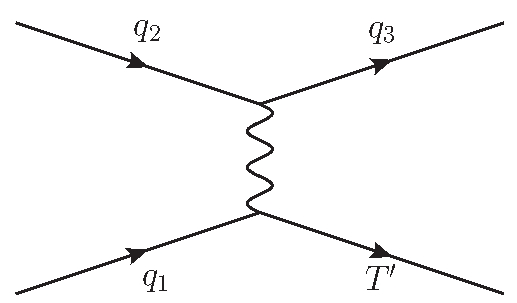
\includegraphics[width=0.9\textwidth]{../figs/Tchannel_T_single.jpg}\\
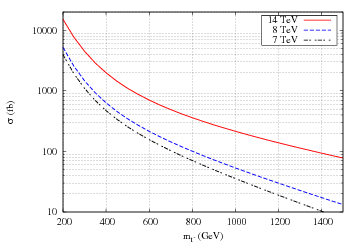
\includegraphics[width=1.05\textwidth]{../figs/pheno_prod_single_tp.png}
\end{center}
\end{column}
\end{columns}

\end{frame}